\documentclass[a4paper,11pt]{article}

\usepackage[english]{babel}
\usepackage[utf8]{inputenc}
\usepackage{amsmath}
\usepackage{graphicx}
\usepackage{xcolor}
\usepackage{cite}


%%%%%%%%%%%%%%%%%%%%%%%%%%%%%%%%%%%%%%%%%%%%%%%%%%%
% Students with dyslexia can use an alternative font. To do so, remove the % symbols in front of the three \usepackage commands below.

%\usepackage[T1]{fontenc} 
%\usepackage[bitstream-charter]{mathdesign}
%\usepackage[scaled]{helvet}

%%%%%%%%%%%%%%%%%%%%%%%%%%%%%%%%%%%%%%%%%%%%%%%%%%%

\setlength{\oddsidemargin}{0cm}
\setlength{\evensidemargin}{0cm}
\setlength{\voffset}{-2.5cm}
\setlength{\textwidth}{16cm}
\setlength{\textheight}{25cm}

\title{{\small PHY480 Semester I Project Report}
\\
\vspace{5mm}
Machine Learning and Categorising Objects in the Sky}

\author{160207219}

\date{\today}

\begin{document}
\maketitle

\begin{abstract}
This is the Semester I Report for the fourth year project on Machine Learning and classification. There are three sections to this report. First I conduct a literature review to show the history and development of the field, as well as identify possible routes of research. Second, I detail my progress in the project during semester I. Third, I lay out the further plans for this project in the second semester.\\

\end{abstract}

\section{Introduction}
This project is based on the need to classify astronomy objects from the Gravitational Wave Optical Transient Observatory (GOTO). Such classifiers have already been done for images from other sky surveys like SLOAN digital sky survey. However, this project is primarily focused on applying existing techniques to this dataset. The primary classification is to differentiate between stars and galaxies. If time permits, an attempt will be made to classify between different types of galaxy (Spiral, Elliptical, Irregular).

This project will comprise two parts: a source detection algorithm must be developed to extract astronomical objects from the images provided. And the machine learning section proper, which classifies those images. 



\section{Literature Review}
Throughout astronomical history, there was a great need for the classification of objects, be it determining whether the objects are nebulae or stars, or differentiating between different types of galaxies. However, given the vast amount of data from observations, classifying objects is incredibly costly in terms of human resources. Even from the low resolution images of early photographical plates, one of the most time-consuming aspects of data analysis was to identify which objects are important and of those, which are the type of objects researchers are most interested in. Hence, historically, it was difficult to take advantage of the full range of observational data.

However, with the advent of data processing by computers, it has become possible to process ever larger sets of data while maintaining the same level of human resources. This started the process of developing and using various computerised methods to classify data gleaned from observations. This literature review will detail the methods used, from the most primitive methods, to the latest developments in neural networks, of how astronomical objects became classified.
\subsection{Early Methods of Classifying Astronomical Objects}
From the beginning of astronomical observations, it was determined that some objects are more like others, and hence a classification system was developed. Since the earliest observers had no way of reliably recording their observations—they used hand sketches, there was no real need to have mass categorisation of astronomical objects. All that changed, however with the advent of photography. At the turn of the 20th Century, photographic plates were used to conduct sky surveys and hence build star catalogs. This increased the need to devise some kind of classification scheme to make sense of the objects. Such classification schemes can be seen in the Draper System \cite{russell_1935_the} , or the Hubble Tuning Fork \cite{hubble_1926_extragalactic} . However, applying such schemes to the objects seen on the sky remained a human endeavour. It would remain so until the 1980s where computing technology advanced to a point in which automated classification became feasible.

In 1988, Adorf \& Meurs applied a classification algorithm to the IRAS catalogue data of extragalactic sources.\cite{adorf_1988_supervised}  They made use of AutoClass, a popular machine learning  algorithm at the time. Importantly, they identified two aspects of classification: exploratory and confirmatory. They noted that given a completely unknown set of data, it is much more difficult to make any classification given that one does not know anything 'about' the data—this is exploratory classification. In contrast, confirmatory classification is where one does know the categories that the data must be separated into and therefore the algorithm is just an exercise in the classification of this data, and hence confirming or denying any hypotheses made about the data. From this, it is clear that to do the former, an unsupervised method is needed to determine the underlying structure of the data, however for the latter, unsupervised or supervised methods will work. 

A few years later, a method that could be considered recognisably modern was used to classify the POSS-II sky survey into stars or galaxies.\cite{fayyad_1993_applying} The method starts by performing basic image processing and identifying the sources that need to be classified. The method used is similar to methods used today in the sense that the images processed using a source detection algorithm, and each of the sources would be extracted from the image. Each source then has 18 what they call 'base-level attributes'—what we would call 'features' today—that need to be selected from the source image. These attribute include things like core luminosity and orientation. The attributes for each image are calculated algorithmically and requires no human intervention. However, the attributes themselves are what the researchers determined as important based on their understanding of classifying astronomical sources. While this may make sense prima facie, this is quite a primitive method when compared to modern approaches. The reason because part of the allure of using machine learning is that one can easily stray into the exploration aspect of data science, i.e. using a computer to make sense of data where humans are lacking. While the classification between stars and galaxies may be sufficiently distinct to decide that there is nothing to be gained from allowing a computer to analyse the data sight unseen, that may not be the case when dealing with more subtle classifications, such as those between galaxies types. The algorithm also made use of 'sure-thing stars'. These were stars that were hand picked by astronomers within the dataset that were surely stars. This was the beginnings of the creation of a training set. The SkICAT algorithm—the algorithm developed in this paper—achieved accuracies of 60-80\% between images—when the training set and the test set are derived from different images, and over 90\% within images—when the training set and the test set are derived from the same image. This is a far cry from modern accuracies (up to 95\% over all images; see below), but is an achievement considering the status of computer science research and hardware of the day.
\begin{figure}[ht]
\centering
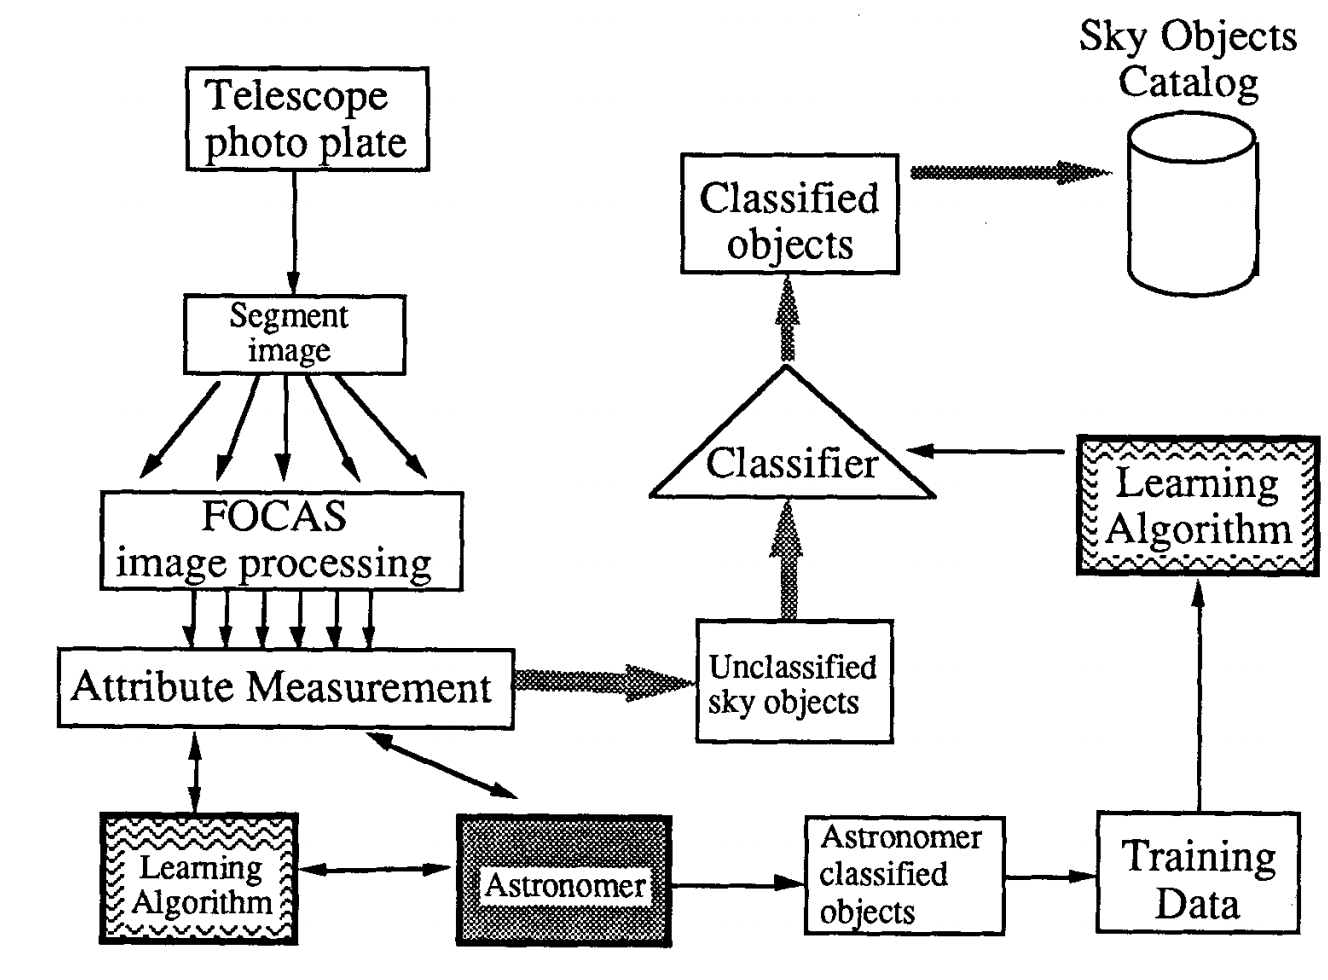
\includegraphics[width=\textwidth]{SkICAT.png}
\caption{\label{fig:SkiCAT}Diagram of the SKICAT algorithm. Note especially that the learning process is inextricably linked with the human astronomer. This method heavily relies on human intervention. \cite{fayyad_1993_applying}}
\end{figure}

Further developments in this vein came from Abraham and Merrifield in 2000.\cite{abraham_2000_explorations} They applied largely the same method of manually identifying features and then classifying the images according to them. However, instead of classifying galaxies into categories, they placed them in a two dimensional 'Hubble Space' in which one axis is the early/late type classification (cf. Hubble Tuning Fork), and the other is the strength of the bar. In doing so, they found that the distribution was not uniform and there were groups of galaxies such as ellipticals, spirals and barred spirals. This matched what was already known at the time—that Elliptical, Spirals and Barred Spiral galaxies are the main types of galaxies. They then classified these galaxies according to these groups. What they  performed was dimension reduction followed by a primitive method of clustering. Clustering is a machine learning tool used to identify the 'clusters' in data. Clustering is an unsupervised method because it does not require humans to indicate what the clusters should be. In this case though, the researchers manually determined features which made the Clustering semi-manual. In this case it is difficult to determine whether the resulting groups are a result of choosing the two parameters because the two parameters chosen are early/late type and the degree of the central bar respectively. One could almost expect to yield these results if one chose those parameters in such a way. Hence, it is unclear from the data whether that is a true classification of galactic morphology, or if it is merely an artefact from the choice of parameters.
\begin{figure}[ht]
\centering
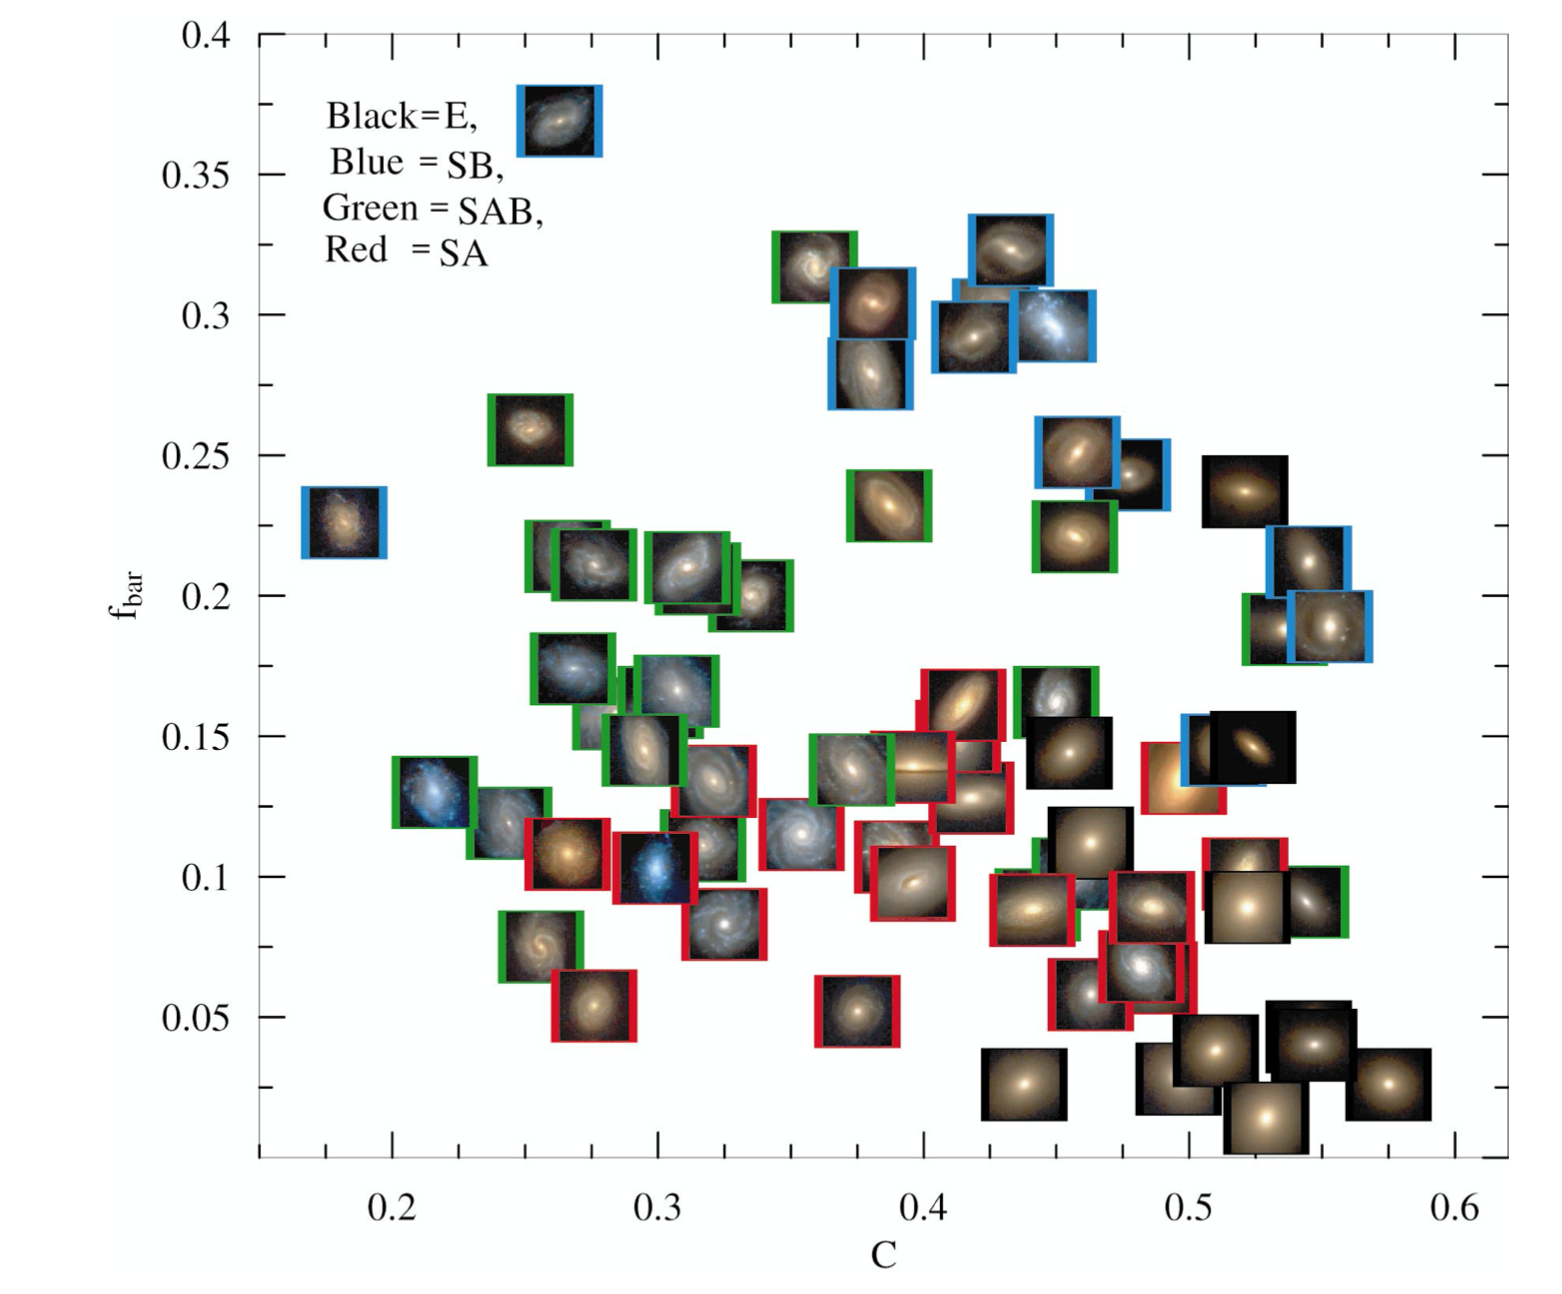
\includegraphics[width=\textwidth]{Abraham.png}
\caption{\label{fig:Galaxies}The distribution of galaxy images in their sample within Hubble Space. Note C represents the early/late type of the galaxy, and $f_{bar}$ represents the prominence of the central bar. \cite{abraham_2000_explorations}}
\end{figure}

\subsection{Support Vector Machines and Principal Component Analysis}
Support vector machines (SVM) and principal component analysis (PCA) are developments in the field of machine learning that have been applied to astronomical classification. SVM classifies the data into two categories using a rather simple but still effective algorithm. This is particular useful for classifying objects which have two classes (Stars and galaxies, spiral and elliptical galaxies, etc) hence it has been the classifier of choice for astronomical purposes. PCA is a method of dimensionality reduction. Since the source images for which classification has to be performed has many features (each pixel can be considered an individual feature). There was (and still is, in some cases) a need to reduce the very high number of features of the data. Since each feature corresponds to a dimension in the data, and computational time is almost always follows either a power law, exponent, or polynomial proportionality to the features, it is greatly desirable to reduce the dimensionality of data as much as possible.
\subsubsection{Support Vector Machines}
In order to understand support vector machines (SVM), one must first understand the earlier logistic regression algorithm. Logistic regression operates on a sample by separating it into two classes. It makes use of the logistic function:
\begin{equation}
h_{\theta}(X)=\frac{1}{1+e^{\theta^{T}X}}
\end{equation}
where $h_\theta (X)$ is a 'generalised linear parameter'. What a generalised linear parameter is not important for the discussion of logistic regression, but a generalised linear parameter is used because in machine learning, operations are performed by vectors and matrices. All these operations necessitate that whatever is the result of them, it must be either a vector or a matrix, which is why a linear parameter cannot be used and must be generalised, in this case, the generalised linear parameter is a matrix. The key effect of logistic regression is that any such 'dividing' line (or hyperplane when there are more than 2 dimensions) that successfully splits the parameter space in two according to the training data is a 'good' split. However logistic regression gives no indication on how good a particular fit is. That is the motivation for developing SVM.

Without getting into the specifics of the algorithm, when training either logistic regression or SVM, a cost function must be found. The cost function in the logistic regression is smooth while in SVM is a hinge loss. A hinge loss is a loss function which has a constant value somewhere, and a function elsewhere. In the case of SVM, the function has 0 when a datapoint is on the 'right' side of the hyperplane (i.e. classified correctly), and a linear function depending how far it is from the hyperplane when it is not. This enables it to measure the 'goodness of fit' as the further a point is wrongly classified, the greater the loss function is. SVM tries to maximise the margins between the hyperplane and the closest data point to either side of it. This is useful in many cases because SVM gives the 'best' classifier in some description of the word. Contrast this with logistic regression, where any classification would be accepted by the algorithm as long as all the data points are are on the right side, SVM would maximise the distance between the nearest point and the hyperplane, thereby leaving only one classification that is the 'best'. 
\begin{figure}[ht]
\centering
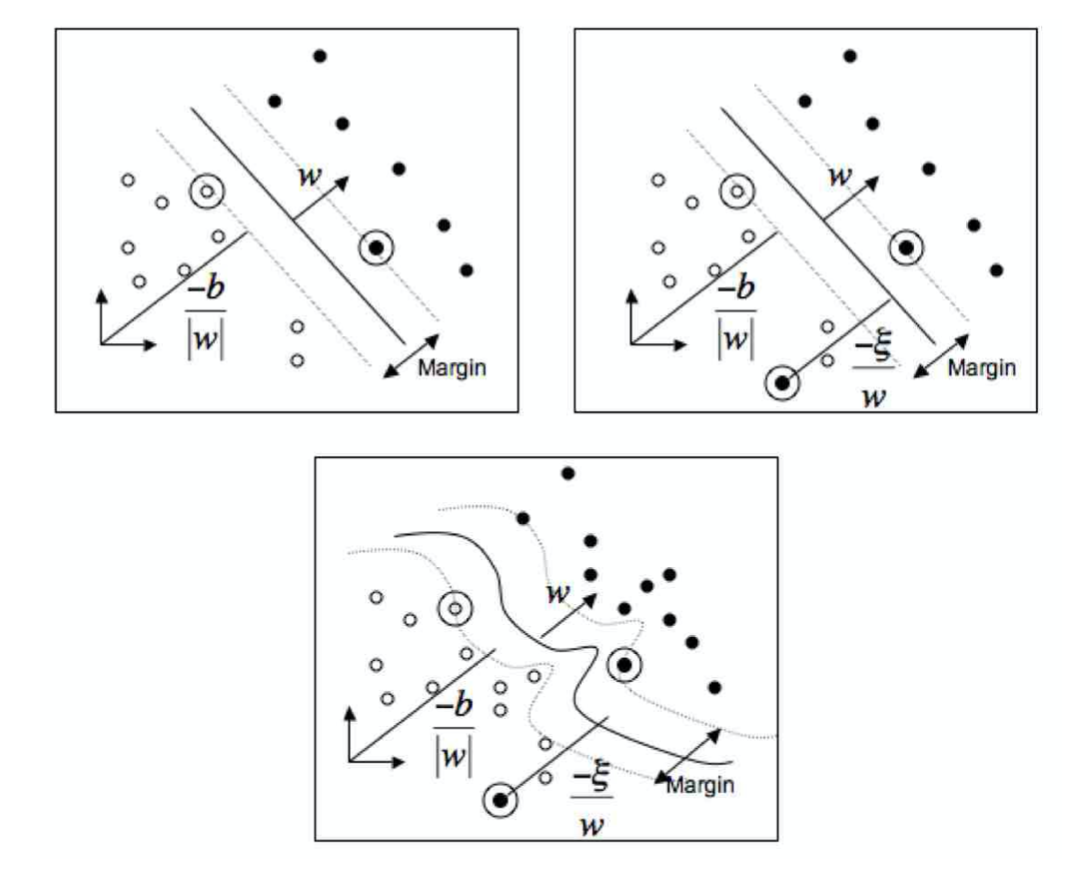
\includegraphics[width=\textwidth]{SVM.png}
\caption{\label{fig:SVM}A figure showing how SVM works. The upper left shows SVM with linearly separable data. The dashed lines represent the parallel distance (w) which represents the distance from the closest point to the dividing line. This is the margin (2w), as labeled. The upper right shows SVM with non linearly separable data. The black dot on the wrong side of the fit would represent a large contribution to the loss function. The bottom shows kernel SVM with non linearly separable data. This classification is clearly still an SVM classification, given the two dashed lines, but given it is not linear, it must be some kind of kernel SVM algorithm. \cite{huertascompany_2010_revisiting}}
\end{figure}
\subsubsection{Principal Component Analysis}
The motivation of principal component analysis (PCA) is to reduce the dimensionality of data while preserving as much information as possible. This is useful because reducing the dimension of data makes it much less computationally expensive to manipulate and analyse it. The underlying theory of PCA is beyond the scope of this literature review, but in broad terms, PCA makes use of matrix manipulations to find the eigenvalues/eigenvectors of the matrix of data. This is then further manipulated to give a set of components (so-called principal components), which are sorted in accordance to how much of the information they retain from the original data. The first component will have most of the information and the second will have less, and so on. If one chooses to truncate the components at some value, one can still be certain that they will have 'most' of the information retained. This tool is greatly useful because it is not very computationally expensive, with computational complexity of $O(\min(p^3,n^3))$ \cite{johnstone_2009_on}, where n is the number of data points (sources, in the specific case of astronomical classification) and p is the number of features. However, this method loses meaning on the specific components resulting from the algorithm because each principal component is some linear combination of all the original components. This is particularly unhelpful when the original components are meaningful—consider a situation where a medical researcher used data to try and calculate the risk of cancer using a high number of medical parameters (blood pressure, body weight, etc). He performs PCA and after classifying, he finds that one particular principal component correlates heavily with cancer. However, because of the nature of PCA, none of the principal components correlate cleanly with any of the initial parameters, which would reduce the effectiveness of identifying the component. However, in the case of astronomical classification, each feature to begin with is not meaningful in itself. Most of the time it is simply the intensity of light for a particular pixel in the detector. Hence, where was no need to trace the classification of objects to any particular value in a pixel, PCA does not lose insight this way when used for this purpose.
\subsubsection{SVM and PCA as applied to astronomical classification}
SVM and PCA started to be applied to astronomical classification in the early 2000s. The work of Calleja and Fuentes was one of the earlier applications of PCA to astronomical classification.\cite{delacalleja_2004_automated} They used PCA and a variety of classification algorithms to classify galaxies from the SDSS. 8, 13, and 25 principal components were used to perform their classification because they represent 75\%, 80\%, 85\% of the information from the data. Note how the marginal benefits of including many more principal components are diminishing as a result of PCA. They made use of a number of classifiers, with a Random Forest classifier being the best. They found that when classifying into 3 classes the accuracy is 91.64\%; 5 classes: 54.72\%; 7 classes: 48,62\%. This indicates that there are probably 3 'true' classes in the data. However this is not known until further clustering analysis is performed.

Conselice \cite{conselice_2006_the} found that, using a sample of over 20000 galaxies, the principal components extracted using a PCA analysis on the sample largely matched what was predicted from astronomical understanding. He found that the 3 main components are scale, star forming regions, and galaxy interactions/merger. From this, he developed a 3 axis classification of galaxies. However, he notes that real galaxies are much more 'messy', and this is one of the key points from this paper \cite{conselice_2006_the} —real life objects do not fit cleanly into categories assigned. Therefore, it is quite possible that objects are simply unclassifiable or are otherwise not suitable for the classification system assigned, hence, the blind pursuit of 100\% accuracy is ill founded and inadvisable.

Huertas-Company et al \cite{huertascompany_2007_a} wrote two papers on using SVM to classify galaxies. They reduced the data down to 12 parameters and performed SVM on them. The classification was performed to separate them into two groups—early and late types. They found that with the WIRCam (Wide-field InfraRed Camera) sample, the accuracy only reached 60\% while for the better SDSS sample, the accuracy reached 80\%. The accuracy for SDSS appears to be better because the quality of the data (in terms of noise and resolution) is higher in SDSS compared to WIRCam. Also, this is to be expected as the 12 parameters for the galaxies do not seem to be linearly separable. When some of the 12 parameters are related to each other, the information gleaned from the 12 parameters is somewhat reduced by the covarying parameters.

In their subsequent paper \cite{huertascompany_2010_revisiting}, the group used a SVM classifier to classify the data. They attempted to further classify the two classes (early- and late- type) and therefore split each of the classes into two; ultimately forming 4 classes: E, S0, Sab, Scd. From their paper, it was apparent that the pre-built classifier was performing a 'kernel-SVM', or using SVM with a 'kernel trick'. This trick transforms the originally linearly inseparable data to a higher dimension using the eponymous kernel. This allows the data to be linearly separable in some higher dimension. (See figure 4. This concept is much easily explained in an image rather than in words) In fact, the mathematics guarantee that there are an infinite number of kernels which can be used, and at least one of them is linearly separable (gaussian kernels map the data to infinite dimensional space, which makes the data linearly separable). 
\begin{figure}[ht]
\centering
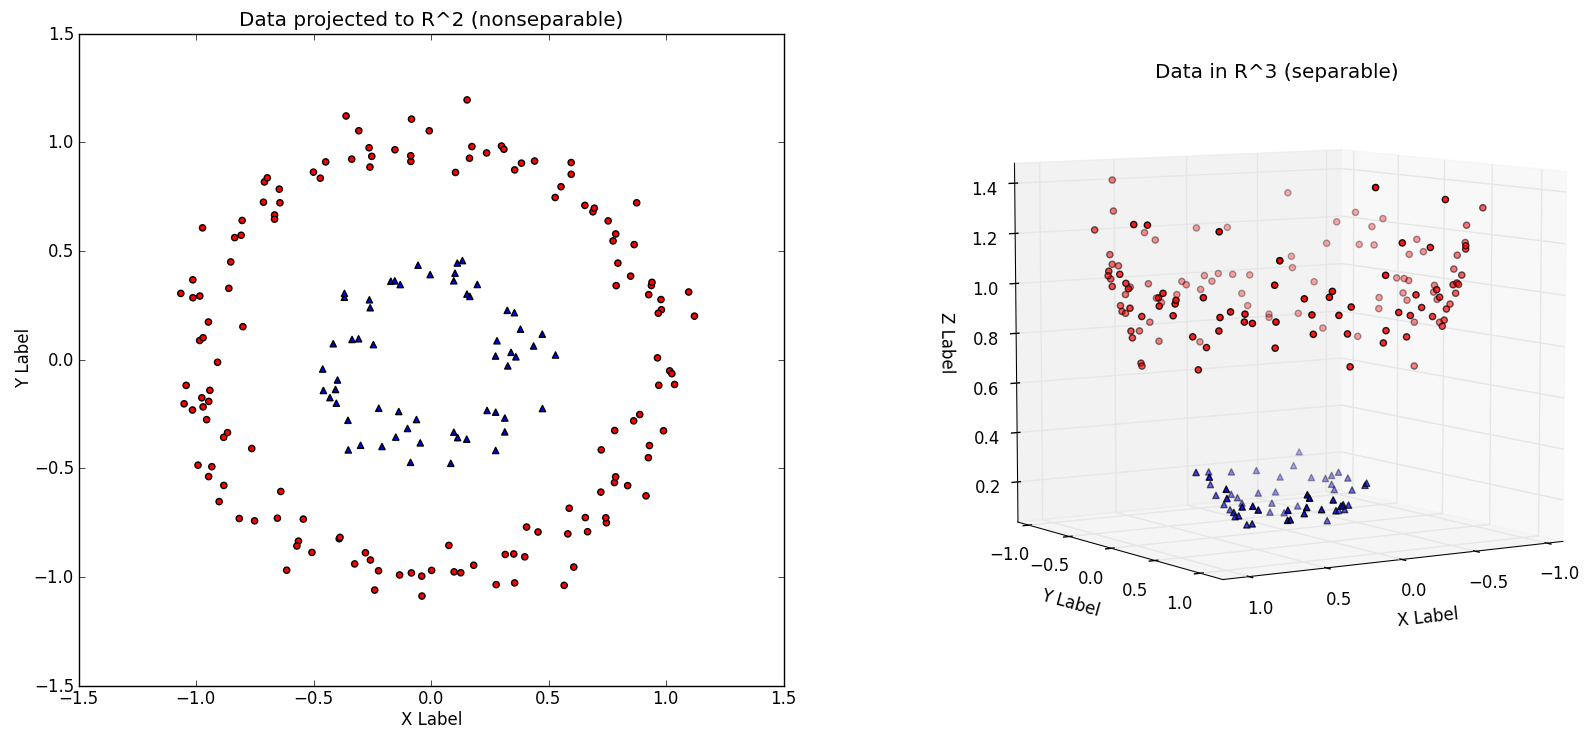
\includegraphics[width=\textwidth]{kernelSVM.png}
\caption{\label{fig:kernelSVM}When data is mapped to a higher dimension, it might make it linearly separable when it previously was not. The data on the left is mapped into the 3 dimensions, which is the right image. While in 2D the data is not linearly separable, in 3D it is apparent that it may be done.\cite{saptashwabhattacharyya_2018_understanding}}
\end{figure}

The group \cite{huertascompany_2007_a} , using kernal-SVM achieved greater success in their classification, with a scatter of 12\%, it may be assumed that their accuracy was 88\%. Scatter is a parameter which quantifies how much of the data does not match the classification, while the paper does not detail what definition of scatter they use, from the text it seems that matches what I have been calling 'accuracy'. They also mentioned that 0.4\% of objects were considered unclassifiable.  

This shows the power of a relatively old method—SVM—which can be updated to compete with more modern methods, and this may be a way forward in binary classifiers.

\subsection{Neural Networks}
Neural networks are so termed because they are similar to the way neurons in the human brain work. There are several types of neurons in neural networks, but broadly speaking they perform simple calculations, pass the information forwards or backwards, and retain the information for a period of time. When these neurons are combined, they form neural networks (NNs). 
\begin{figure}[ht]
\centering
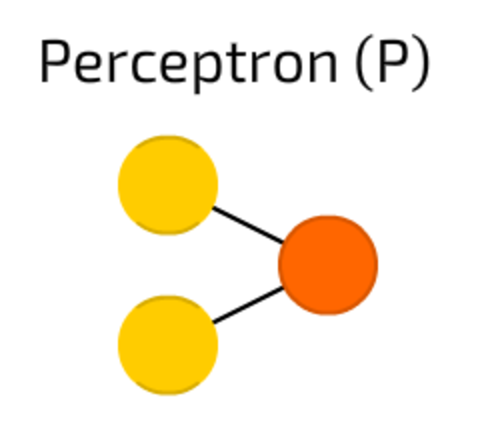
\includegraphics[width=0.25\textwidth]{Perceptron.png}
\caption{\label{fig:Perceptron}A Perceptron is the simplest neuron. It takes in numbers and performs a sum. They may be simple classifiers. \cite{tch_2017_the}}
\end{figure}
\subsubsection{Artificial Neural Networks}
Artificial neutral networks (ANNs) are not a type of neural network per se. Rather, they stand in contrast with the convolutional neural networks that will be discussed later. ANNs are so termed because they make use of a neural architecture that is pre-determined. All ANNs require features to be selected beforehand, by a human, or by an algorithm like PCA. The simplest of these ANNs is the feedforward neural network (FNN). The concept of an FNN has existed since the 50s, but they are not very useful since they only have one layer—a single layer FNN can only classify linearly separable data, which is not very useful given SVM can do that too.
\begin{figure}[ht]
\centering
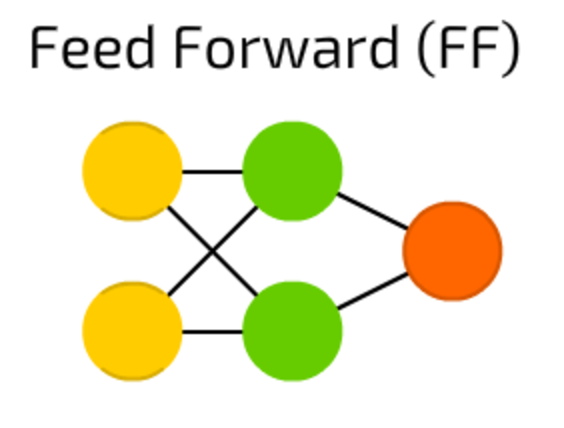
\includegraphics[width=0.25\textwidth]{FNN.png}
\caption{\label{fig:FNN}A FNN comprises of a fully connected network that only passes information forward. \cite{tch_2017_the}}
\end{figure}

The FNN concept can be easily extended by increasing the number of layers between the input and the output layer. A FNN that has more than one layer is called a Deep FNN (DFNN). 

\begin{figure}[ht]
\centering
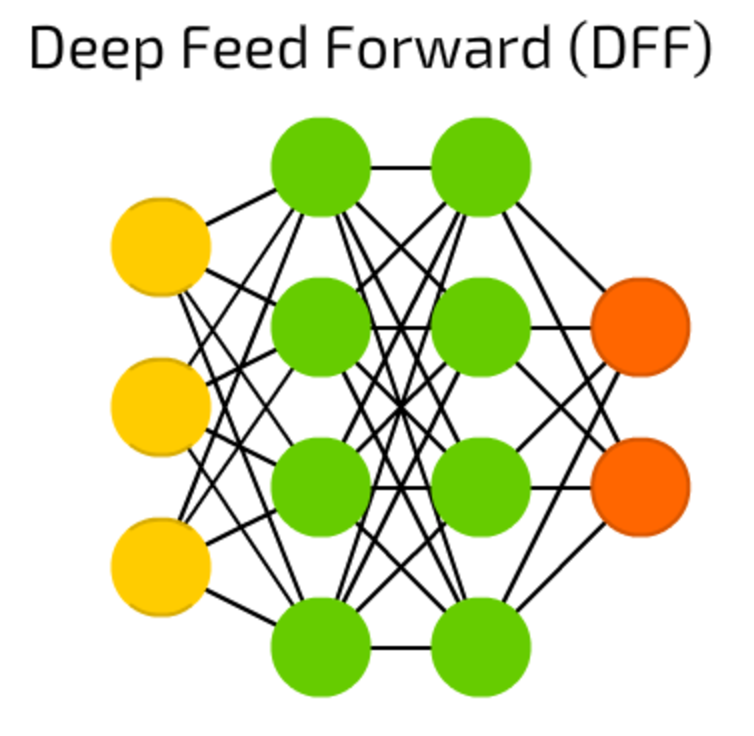
\includegraphics[width=0.25\textwidth]{DFF.png}
\caption{\label{fig:FNN}A DFNN is simply a FNN with more layers. It retains the characteristics of being fully connected and information only passed forwards.\cite{tch_2017_the}}
\end{figure}

The DFNN arose in the 90s, where the methods to train them finally existed—previously, because of the nature of error propagation, errors would accumulate through the network and eventually cause the network to fail entirely. One such method developed is to use 'leaky' nodes, in which some small portion of nodes will be automatically set to 0. This has the effect of dampening the effect of errors. Now, it is used in lieu of the simple FNN and produces superior results—both in terms of allowing for classifying non-linearly seperable data, but also because the more nodes allow for higher maximum accuracy.

Another type of artificial neural network that is relevant today is the recurrent neural network (RNN). A RNN is in essence a FNN with the nodes replaced by recurrent nodes. A recurrent node is simply a node which feeds itself as an input to itself after a time-delay. 
\begin{figure}[ht]
\centering
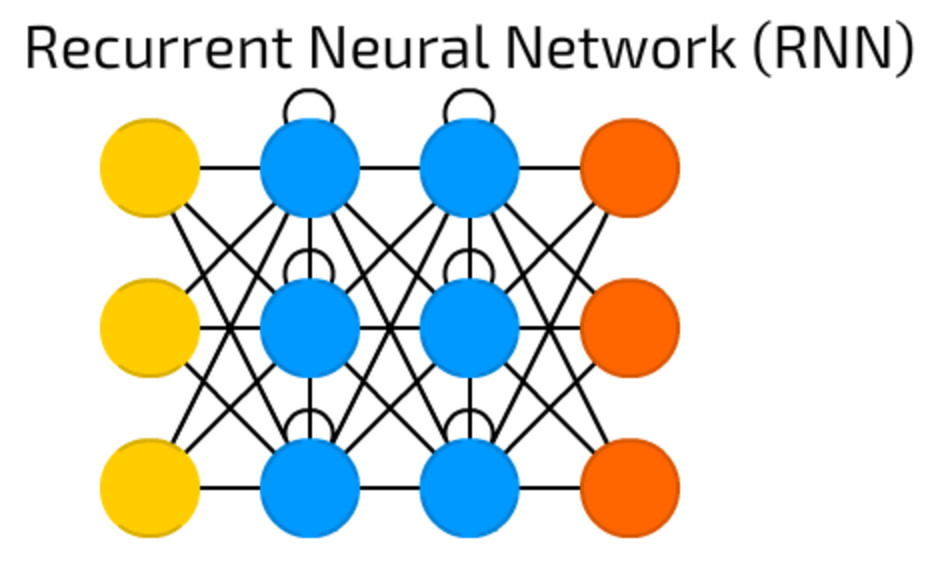
\includegraphics[width=0.25\textwidth]{RNN.png}
\caption{\label{fig:RNN}An RNN is very similar to an FNN, in fact it has the same structure except it changes the nodes from only feeding forward to being recurrent.\cite{tch_2017_the}}
\end{figure}

RNNs are used today in applications where context is sensitive, like natural language processing—a word said is inherently linked to the word said before it, so in natural language processing, giving the neural network information about the previous word is useful. However, given the nature of astronomical images, this does not seem like a viable or useful path.

Because convolutional neural networks  are inherently more suited to image processing (as will be explained), work on the field of applying ANN to astronomical classifications is very limited. The only work on the field seems to be to classify spectral data—because spectral data is not imagery in nature.\cite{hampton_2017_using} 

\subsubsection{Convolutional Neural Networks}
Convolutional neural networks(CNNs) are structurally very similar to FNNs, the difference here is that the activation functions of those nodes are not simple activation functions, but rather convolutional and pool activation functions. Convolution layers are nodes which convolve the images. This entails passing a convolutional filter, which essentially just 'looks' at the image in smaller sections. Then this outputs the convolved image into the next node. Figure 10 is a good depiction of this. 

A pooling layer reduces the spacial size of the network by essentially downsampling the resultant from the previous convolutional layers (A very good non-technical analogy is the downsampling of 4K video footage to 1080p footage. Essentially every 1 in 4 pixels are used to bring the resolution down). This step is necessary because it reduces computational complexity and also reduces overfitting.
\begin{figure}[ht]
\centering
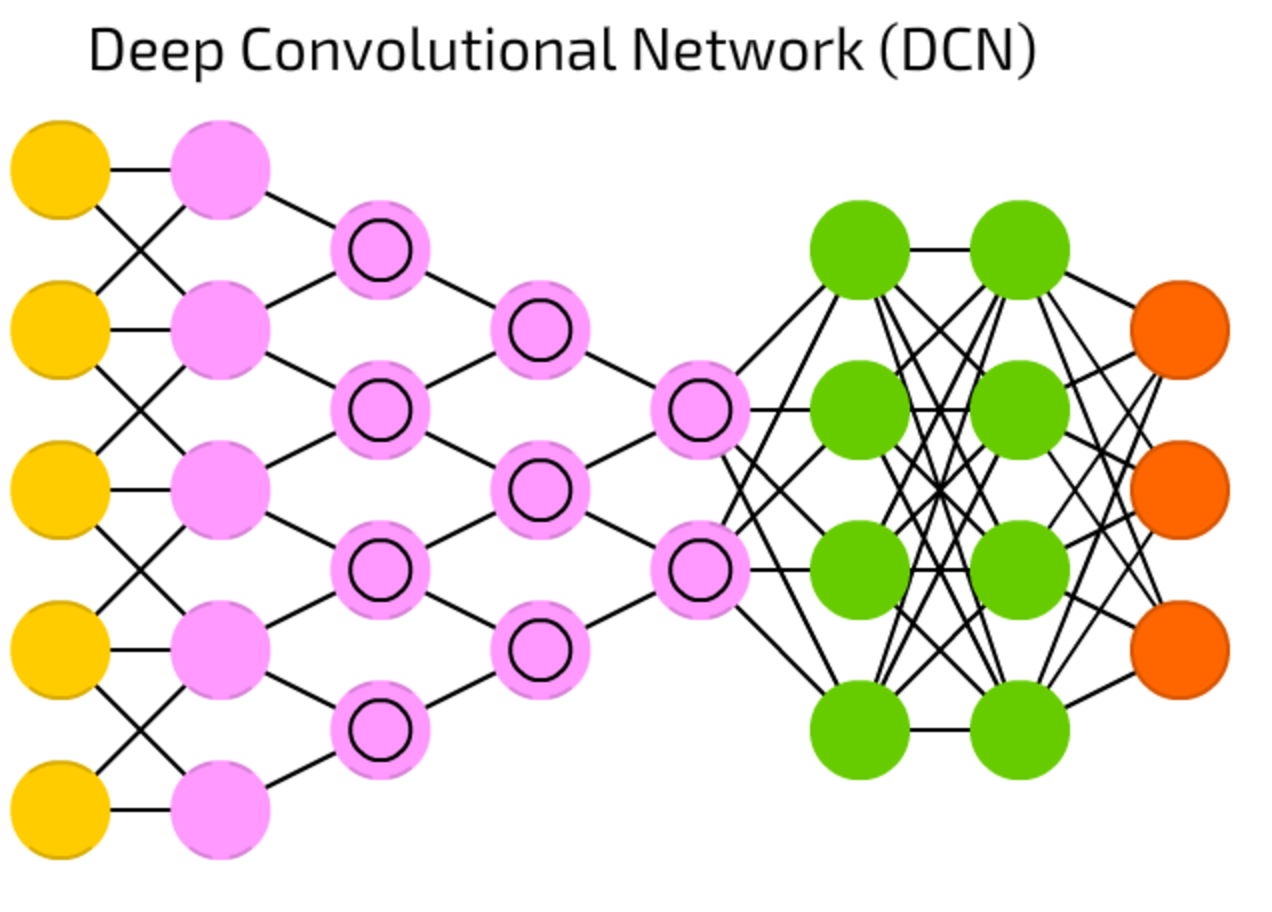
\includegraphics[width=0.25\textwidth]{CNN.png}
\caption{\label{fig:CNN}A CNN uses convolution and pooling layers instead of feedfoward nodes. Note that FNNs are frequently used at the end of CNNs for further data processing.\cite{tch_2017_the}}
\end{figure}

However, in practice this is very different. Since convolution functions act on images rather than specially selected features, they avoid the process of selecting features from the images.

CNNs have been extensively used in galaxy classification since the late 2010s. There are various approaches using a differing combination of convolutional hidden layers (nb. hidden layers are all layers except the last one because one does not interact with these layers, and are hence 'hidden' from view) and pooling layers as well as varying levels of hardware capability. Kim \& Brunner \cite{kim_2016_stargalaxy} made use of 5 band images to classify galaxies. They used a structure with 8 convolutional layers, 3 pooling layers and 2 fully connected layers—fully connected layers are essentially FNNs. They achieved an accuracy of 95-98\% depending on which accuracy metric is used. However, in their discussion they mentioned that there was a lack of training data to train with, and this seemed to be a problem which is shared with others working with CNNs. \cite{khalifanoureldeenm_2017_deep} \cite{aniyan_2017_classifying} The reason for this seems unclear to me as there is not a dearth of astronomical data, in fact there is a wealth of such data, why they are not able to acquire such data is quite curious to me. A possibility is that while astronomical data is indeed plentiful, labeled data which is required to create a training set might be meagre. 
\begin{figure}[ht]
\centering
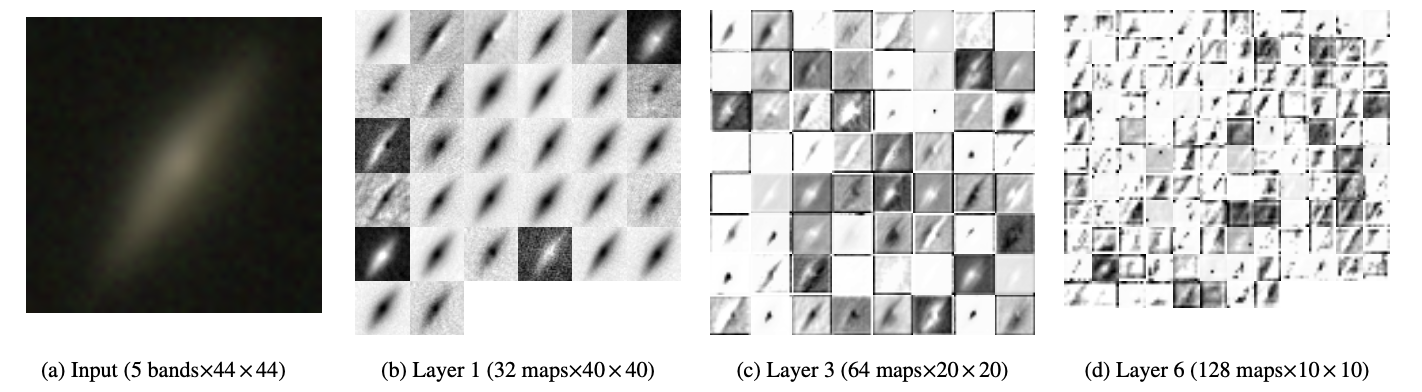
\includegraphics[width=\textwidth]{CNNExample.png}
\caption{\label{fig:CNNExample}An image taken from the Kim paper which demonstrates how a CNN works: by repeatedly passing the original image through a convolving filter to make sense of the image. Note how the image is being separated into more an more maps, which are aspects of the image (such as corners and edges), via convolution. This process increases the number of maps but decreases the spacial size of the image. \cite{kim_2016_stargalaxy}}
\end{figure}

From the literature, it is also quite clear that there are not too many astronomers truly using CNNs for classification, rather, it seems the wealth of literature is of computer scientists using astronomy data as a proof of concept for their CNNs. \cite{khalifanoureldeenm_2017_deep} And these all garner results of over 95\% with very little data. However, the benefit of computer scientists doing the research is that their code is more freely available on repositories such as GitHub.

The path of CNNs seem very promising if one has sufficient data, and labeled data is not lacking in this project. 

\subsection{Galaxy Zoo}
When training neural networks, copious amounts of training data is needed. One method of acquiring such training data is through sky surveys, but another is through citizen science projects like Galaxy Zoo. \cite{lintott_2008_galaxy}

The Galaxy Zoo project was a massive project which harnessed the power of mainly non-professional astronomers to classify images from sky surveys. The accuracy of those classification collectively are on par with the best neural networks. Further, the classified data is freely available online, and therefore is easily used as training data. This approach has already been tried by some groups. Banerji has used Galaxy Zoo data to train a neural network and achieved 90\% accuracy. \cite{banerji_2010_galaxy} However unfortunately he does not specify what kind of neural network they are using—they call it an artificial neural network, but it is unclear if they are under our definition(ANNs have an alternate definition which includes CNNs and essentially includes any neural networks) or if it is as it appears that they are using some kind of decision tree—and so it is impossible to verify whether the accuracy is due to deficiencies in their neural network or in the Galaxy Zoo data. 

\subsection{Exotic Methods}
There are more exotic methods attempted in the literature to classify galaxies. One of which is Hocking et al \cite{hocking_2017_an} , who used a 'neural gas' in an unsupervised classification algorithm. They attempted to replicate findings by the Galaxy Zoo Project in the CANDELS field. They discovered that the classifications somewhat matched what a human classifier would identify in terms of early/late type galaxies. Such unsupervised methods had also been attempted earlier by Schutter \& Shamir, \cite{schutter_2015_galaxy} albeit to somewhat less success—they gave their final result as having galaxies classified they way they did was less than $1.53 \times 10^{-12}$. But it is unclear how this translates to the more familiar language of accuracy values.

Another method which is equally exotic is Abd Elaziz et al. They used an artificial bee colony to classify galaxies. \cite{abdelaziz_2018_galaxies} The artificial bee colony is an algorithm based on the concepts of Gegenbauer moments and it is somehow related to the way real bees interact. The mathematics involved is highly complex and is frankly beyond me. The results were comparable to using SVM when only 150 features are accounted for. When all features are used, SVM outperforms the artificial bee colony.

\begin{figure}[ht]
\centering
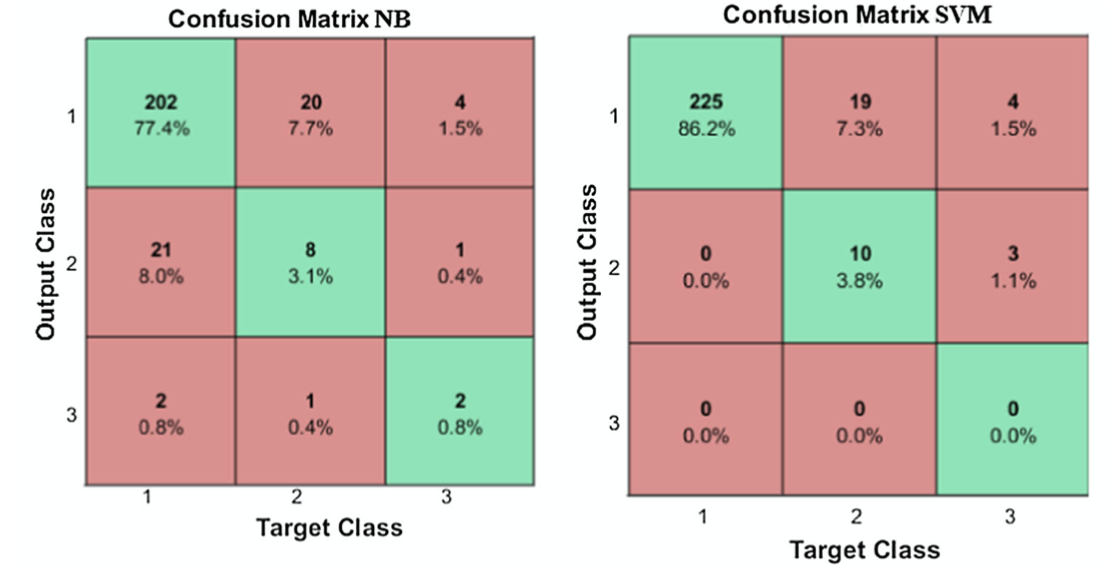
\includegraphics[width=\textwidth]{confusion_matrix.png}
\caption{\label{fig:CNNExample}The confusion matrix from the Artificial Bee Colony compared with an SVM approach. Note that it seems SVM is superior when all features in involved. \cite{abdelaziz_2018_galaxies}}
\end{figure}

However, the point of these exotic methods is not necessarily to be immediately applicable, but they may drive new developments in the field generally that may one day be somehow applied to astronomical classifications.

\subsection{Summary}
The use of machine learning to classify astronomical objects is still a rather new development. The field has developed tremendously from the original crude methods of determining stars from galaxies using a centroid of the source. Through using manual assignment of features to using PCA to automate this, we have gained the ability to gain insights into data we could not previously. The advent of SVM in the adjacent field of computer science yielded a more effective algorithm at classification. And within the past 5-10 years, the use of neural networks is being developed rapidly.

With respect to the task at hand—classifying between stars and galaxies, a revising of SVM, more specifically kernel SVM seems warranted. Using CNNs may also bear fruit in this endeavour, although that may be less efficient than a simpler algorithm like SVM. However, in the case of classification of galaxy types, CNNs look like the proper approach.

It is also apparent in the literature that there is a dearth of labeled data for training purposes. It is possible that the way forward in the field entails some kind of unsupervised algorithm, although that approach would take too long for the current project. 

\newpage


\section{Progress on Project}
Progress on the project has been behind schedule. So far, after completing the literature review, a source detecting algorithm has been created, but that requires the data to be exported from the .fits files into a numpy format, which erases the sky-coordinates among other metadata. This is undesirable because ultimately the sky-coordinates are necessary to cross reference with existing sky surveys to create a training set data. Therefore, an alternate method must be sought. 

In seeking such an alternative method, the code will also be extended to loop through all the training set images as opposed to the current single image. 

In terms of documentation, I have set up a github page which is shared with my supervisor (Dr James Mullaney), in lieu of a standard lab-book. This is more appropriate since given a coding based project, the github page retains all the functionality of a lab book of permanency, but has the added benefit of being designed for the purposes of code. A link to the github page is provided in the appendix.

In addition, I have gradually familiarised myself with the differences between working on a Unix based system (MacOS which I am used to), and Windows NT system (Windows 10) which I need because I would like to make use of Nvidia CUDA cores which are not available on a Mac Machine.

\section{Project Plan}
\subsection{Postage Stamp Cutout}
Small 'postage stamp' cutouts from the large image are required to train SVMs. This requires that the previous source detection algorithm is functional. I believe this will take up to 10 hours. 
\subsection{Cross-Referencing Data}
After a satisfactory set of postage stamps is acquired, the cutouts need to be cross referenced with existing sky surveys to identify known objects to use as a training set. For now, the plan is to use SDSS to be the primary catalogue of reference. This should take up to 10 hours.
\subsection{PCA}
Performing a PCA on the data should be straightforwardly applying the algorithm. The issue is computing time, but I don't foresee this taking a vast amount of that either. I will allocate 5 hours to this for the time being.
\subsection{SVM and Kernal SVM}
Once the PCA is complete, a simple SVM can be performed, either using packaged algorithms or self-written ones. The limiting factor here is also computing time since an SVM algorithm is quite straight-forward to write.
Once that is complete, a kernal-SVM algorithm will be attempted. However since this is quite complex, a packaged solution will probably be used. I foresee many potential issues with trying this so I would allocate a total of 25 hours for this section.
\subsection{CNN}
After the SVM/PCA method is completed, a CNN will be attempted. Since the allure of a CNN is that it does not require the cutting out of postage stamps, that will be the first choice. However, it is still difficult to see how to properly make a training set for CNN this way. Further, many refinements would be necessary for a CNN, and training each iteration will be very time intensive. Therefore, I will conservatively estimate that 60 hours will be needed.
\subsection{Report}
After the project proper is finished, the report will be written. I expect some 10-20 hours will be spent on report writing.
\subsection{Other areas}
If there is any time to spare, other possible areas of work would be to make a Feedforward Neural Network and compare the results to kSVM. Otherwise, if the project proceeds vastly better than expected, an attempt to classify galaxies can be done.
\newpage

\bibliographystyle{apalike}
\bibliography{Semester_1_report}



\newpage 
\begin{appendix}

\section{Relationship to previous projects}
I have previously completed a machine learning summer internship (Summer 2019) in which I made teaching materials for a university course at the University of Hong Kong. However, since it is a general machine learning course with no research component, it can only be described as a good baseline for this project with no suspicion of self-plagiarism.
\newpage

\section{GitHub}
The GitHub site used for this project can be accessed here: https://github.com/kpklo1/Machine-Learning-and-Galaxies

\end{appendix}


\end{document}
              
    
